\label{subsec:case_studies}

We have applied \projectname~to three open source SDN control platforms:
POX~\cite{pox}, NOX~\cite{nox}, and Floodlight~\cite{bigswitch}. We
found \num{several} bugs in total, and were able to localize a minimal
causal sequence in all cases. \colin{Tone this down.} We describe these case studies in detail here.

\noindent{\bf POX empty list removal.} The first controller we examine is
POX~\cite{pox}, the successor of NOX. POX
is a single-machine control platform designed in the spirit of
Onix~\cite{onix} to provide programming
abstractions on top of the low-level details of switch-controller
communication.

We start with a relatively trivial bug to illustrate the range of bugs our
technique can useful for. We employed \projectname~to generate random sequences of
inputs, and found after some time that an exception was thrown in POX. The
exception was caused by attempting to remove an element from a list that was
not actually present.

There were $76$ randomly generated inputs in the trace leading up to the
exception. We invoked \simulator~to identify a two element minimal causal set:
a switch failure followed by a switch recovery. Apparently this particular
input sequence had not been tested before, and \simulator~made it easy to
identify what inputs caused the erroneous code path to be triggered. At the least,
this minimization serves to simplify integration tests for this exception.

\noindent{\bf POX routing loop.} The next bug we encountered was found in
the POX routing application.

\begin{itemize}
\item Floodlight failover re-cap
\item NOX routing
\item POX distribution?
\item Frenetic?
\item A bug where our technique didn't work
\end{itemize}

\subsection{Domain Knowledge}
\label{subsec:domain_knowledge}
\begin{itemize}
\item How much effort did it take to codify domain knowledge? (table with lines of code)
% Include how many lines it took to interpose on the logging library, and how
% many lines it took to answer snapshot requests.

% The logging statements must also contain enough context[d] to allow for
% unambiguous fingerprinting. -> what exactly this means
\item How often do unexpected internal events occur in practice?
\end{itemize}

\subsection{Runtime}
\label{subsec:runtime}

The POX list remove exception did not depend on delicate timings,
and \simulator~was able to isolate the minimal causal set in logarithmic
time. The runtime characteristics of \simulator~for this case are shown in
Figure~\cite{fig:list_runtime}.

\begin{figure}[t]
    %\hspace{-10pt}
    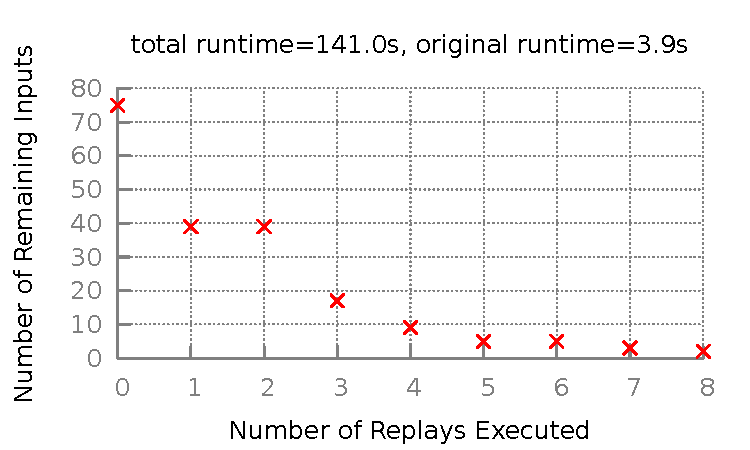
\includegraphics[width=3.25in]{../graphs/runtime/list_remove_error.pdf}
    \caption[]{\label{fig:list_runtime} Minimizing the POX list remove exception.}
\end{figure}

\begin{itemize}
\item Graphs of \# of replays vs. remaining inputs
\item `time compression' benefits
\item Note that runtime doesn't really matter! As long as developer time isn't being used. 
% Scalability:
%We also tested the extreme limits of the simulator's scalability, pushing up
%the number of switches until something broke. We encountered what appears to be
%a limitation of the Linux TCP/IP stack: TCP connection attempts began failing
%beyond 26,680 sockets. Note that 26,680 switches is an order-of-magnitude larger than
%the today's biggest networks.

% Optimizations:
%If the log is too long to rerun from the beginning for
%every iteration, the operator can take causally-consistent
%snapshots~\cite{Chandy:1985:DSD:214451.214456} of the
%live system and bootstrap the simulator from the nearest quiescent snapshot.
%The length of the execution can also be `compressed' by manipulating timers in the
%controllers while still maintaining happens-before dependencies.
\end{itemize}

% ------------------------------------- %
%    OLD TEXT
\eat{

% Just realized: b/c of anonymity, the PC can't chastise us for
% running our system on our own code -- we can't tell them that it's our code!
We applied \projectname{} to three open source SDN control platforms:
Frenetic~\cite{frenetic}, POX~\cite{pox}, and Floodlight~\cite{bigswitch}, and
quickly found (or reproduced) one bug in each. The bug in Frenetic demonstrates
the utility of checking correspondence between high-level policies and
low-level configuration (without needing to specify invariants). The bugs in
POX and Floodlight demonstrate the importance of \simulator{}'s ability to
programmatically prioritize persistent correctness violations and infer their minimal
causal sets.

For all three cases, only a small code modification to the controller was necessary
to retrieve the the platform's state for correspondence
checking.

\subsection{Case studies}

% Outline for bug reports:
%  - Describe each system under test
%  - Describe bugs found
%  - Lessons learned from finding bugs
Here we the discuss the three bugs we found with \projectname{}.

\noindent{\bf Frenetic.} Our first example is Frenetic~\cite{frenetic}, a control platform
providing functional-reactive language
support for programming OpenFlow networks.
Frenetic's language features aim to prevent common OpenFlow programming
errors such as race conditions and overlapping flow entries; Frenetic's
runtime system handles these low-level details on
the application's behalf. Frenetic is a modern SDN controller with a reactive
flow installation policy;
we present it here to demonstrate that \projectname{}, although focused
primarily on proactive controllers, can nonetheless be used to
troubleshoot errors in reactive control platforms.

When running learning switch, the simplest Frenetic application, we encountered
persistent correctness violations immediately. The propagation graph ($\Omega$) for Frenetic's
runtime representation of the network policy had leaves that were not present
in the physical network. Upon closer examination, we found that Frenetic's
runtime system was neglecting to remove old FLOOD routing entries from its
representation of the network policy after the hosts' route had been learned,
even though the learning switch application had
asked for these entries to be removed. Note that this case was not an overtly
malicious bug; the FLOOD entries had indeed been removed from the physical
network. The outdated controller state nevertheless went unnoticed; the bug in
Frenetic's runtime was not specific to the learning switch, and could have
resulted in failure to install flow entries at a later point in time if the
application had asked to re-install them. The key takeaway from this example
is that correspondence checking is a powerful mechanism for
verifying that the controller's representation of the network matches the true
network state correctly; without correspondence checking, troubleshooters
would need to compare the routing configurations and controller's data
structures side-by-side.

\noindent{\bf POX} Our second example is POX~\cite{pox}. POX is modeled after
Onix~\cite{onix}, a production SDN platform; as in Figure~\ref{fig:basicarch}
POX provides a physical view, a virtualized view, and a naive replication
mechanism between distributed control servers.

Because the functionality within POX is relatively young, we chose to
fabricate a bug in POX's distribution failover logic, and independently
validate that the simulator was able to identify, prioritize, and find the
minimal causal set for the fabricated correctness violation.

In particular, we injected the following bug: a controller replica performs
updates to switches by (i) updating the persistent datastore storing the state
of the network (thereby notifying other replicas of the update), and (ii) pushing the
update to the switch. A control server writes a new ACL entry update to the datastore, but crashes
before completing step (ii). The switch is adopted by a new replica,
but the new control server assumes that the state in the persistent datastore
is correct. The ACL entry is therefore never installed in the switch, and a
breach of tenant isolation occurs.

We interleaved this event sequence with a normal system execution trace, and
determined whether \simulator{} could identify the correctness violation.
Throughout the system execution there were a handful of transient
correctness violations overlapping with the isolation breach. Nonetheless, our
simulator was able to identify the correct correctness violation.

\noindent{\bf Floodlight: Distributed controller failover race condition}
We were able to reproduce the problem shown in Figure~\ref{fig:example} in our
simulation environment\footnote{The code is publicly available},
and apply \simulator{} successfully.
We modified the Floodlight software to provide an interface for extracting its
physical view. We did not interpose on internal events of the controller, but instead used a
heuristic to wait for $.5$ seconds between injecting inputs to allow the
controllers to fully react. We ran two of the modified Floodlight controller
instances, connected to two simulated switches, and injected 200 extraneous link
and switch failures, with the controller crash and switch connect event\footnote{We used a switch connect
event rather than a link failure event for logistical reasons, but both
can trigger the race condition} that triggered the blackhole interleaved among them.
On ten repeated runs, the algorithm successfully pruned all extraneous
inputs despite non-determinism in the Floodlight internal events. With full determinism and
interposition, we expect that the algorithm should work well for less
fabricated cases.

\subsection{Overhead}

\colin{Reviewer OB: I would prefer to see a more in-depth analysis of why
correspondence checking is not as heavyweight as, say, conventional
model-checking. Is it the inherent symmetry in data center networks? Can we
assume that there is symmetry?}

In addition to describing bugs, we show that \projectname{} is able
to simulate and check large networks quickly.

\noindent{\bf Record and Replay Overhead.} In contrast to general record-and-replay
mechanisms, the amount of recorded state needed for
high-fidelity replay is tractable. With proactive flow installation,
updates are pushed to routing tables over a relatively long time scale; periodic
FIB snapshots along with a log of link state events, control server
downtime, and host mobility information suffice for our purposes. As a point of reference, the Cisco 7000
core switch model supports a maximum of 128K MAC entries and
128K ACL entries~\cite{cisco7000}. Assuming 36 bytes per flow entry,
(larger than the OpenFlow 13-tuple), each FIB will contain a maximum of 9216
bytes, uncompressed. A datacenter of 100,000
hosts includes roughly 8,000
switches~\cite{Al-Fares:2008:SCD:1402958.1402967}.
Therefore a snapshot of the FIBs of the entire network takes up roughly 74 MB.
The VL2 paper reports 36M network error events over one year over 8
datacenters, which implies 8.5 error events per minute per
datacenter~\cite{Greenberg:2009:VSF:1592568.1592576}.
Suppose we took a snapshot of the FIBs in the network every second.
Then we would need to store roughly 4GB, uncompressed, per minute, a relatively small growth
rate for datacenter logs. This information, in addition to a log of host
mobility events (\eg{} VM migrations) will suffice for our purposes. Note that this is a conservative overestimate.

\colin{Notes from Rean Griffith:
\begin{itemize}
\item total vms in a typical datacenter: 1000
\item migration frequency (migrations/minute): 20 per hour
\item VM spin ups/downs: 150 power ons per hour (see our OSR 2010 paper for
power off estimates)
\item Do we log VM migrations and how does that log grow (I wasn't able to
get any estimates on log-growth data)
\end{itemize}

We had an OSR 2010 paper that provided numbers scaled by the number of
VMs in an installation:
Challenges in building scalable virtualized datacenter management
(http://dl.acm.org/citation.cfm?id=1899941)
}

%To account for host mobility, assume that each server hosts 10 VMs,
%and 1\% of VMs are created, suspended, or migrated every minute. Then 10,000 host mobility events must be
%logged per minute, also a reasonable storage cost. \colin{get real numbers}

%As a point of reference, border routers' working RIB size is
%$\textasciitilde$130MB~\cite{Karpilovsky:2006:UFR:1368436.1368439}.

\noindent{\bf Correspondence Checking Runtime.} Computing the propagation
graph for correspondence checking is equivalent to enumerating
all possible paths in the network, which scales with the diameter
of the network and the number of routing entries per switch \colin{Reviewer
OC: scales how? I suspect it's at least N2}.
The propagation graph for each host can be
computed in parallel however, so the computation is bottlenecked by the serial runtime
of computing a single host's propagation graph.

We show the serial runtime of correspondence checking in
Figure~\ref{fig:hsa_runtime}. For this analysis we generated fat tree topologies
between 2 and 48 pods wide, with pre-installed PORTLAND~\cite{NiranjanMysore:2009:PSF:1592568.1592575}
routing tables in each switch. Each data point is the minimum of three
runs\colin{Reviewer OC: seems to overstate value of approach if maximum is much different} on a single Intel Xeon 2.80GHz core. Note that the number of PORTLAND routing entries per switch scales with the number
of pods in the fat-tree. We excluded the time to convert
flow tables to HSA transfer functions, since transfer functions can be maintained
offline.

\colin{Reviewer OB:  what are the characteristics of the PORTLAND routing
table? If the tables were any different, would the performance of
correspondence checking remain the same, degrade or improve? }

\colin{Reviewer OD: First the paper started generally, then it narrows its
scope to PORTLAND-style datacenters. An accurate abstract would have reflected
this narrowing of scope}

As the figure depicts, even for large networks
(27,648 hosts) the serial runtime of correspondence checking is reasonable for
interactive use. The number of serial tasks to be executed
is the number of hosts in the network squared, disregarding ECMP load balancing.
\colin{reviewer B: correspondence is not being checked. I should be clear
that this is the runtime of generating the propagation on the physical
network, which is an upper bound on the runtime of checking the virtual
network.}


\begin{figure}[t]
    %\hspace{-10pt}
    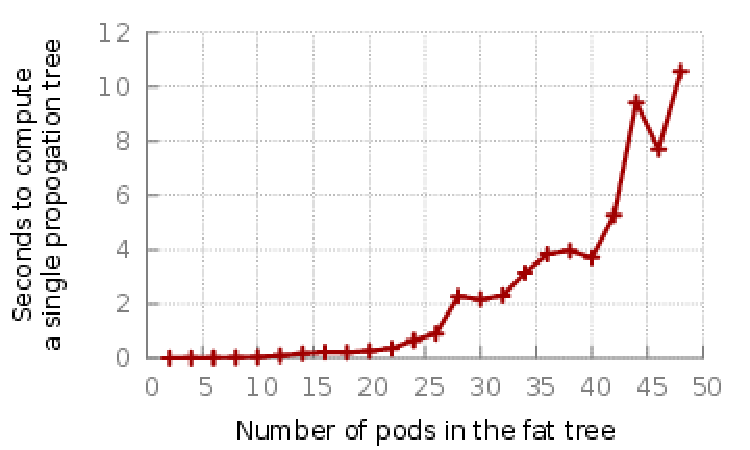
\includegraphics[width=3.25in]{../graphs/hsa_overhead_graph/graph.pdf}
    \caption[]{\label{fig:hsa_runtime} Serial runtime of correspondence
    checking on PORTLAND fat tree networks. Each datapoint consists of
    $x^3/4$ hosts and $5x^2/4$ switches (\eg{} 48 pods means 27,468 hosts
    attached to 2,880 switches)}
\end{figure}

\noindent{\bf Simulator Scalability.} Our design models the entire network
within a single process. We show in Figure~\ref{fig:scalability}
that this approach nonetheless scales to large networks. For this analysis we
generated fat tree topologies between 2 and 48 pods wide, where all switches in
the network connected to a single controller. The controller sent each switch
an OpenFlow
$FLOW\_MOD$ and subsequent $BARRIER\_REQUEST$ message, and waited for the
corresponding $BARRIER\_REPLY$. We then measured the time to between the first
$FLOW\_MOD$ sent and the last $BARRIER\_REPLY$ received. As expected, the
runtime was roughly linear with the number of switches in the network. The
figure also shows that the processing time for large networks (5 seconds per
simulator round) was well within the bounds for interactive use.

\begin{figure}[t]
    %\hspace{-10pt}
    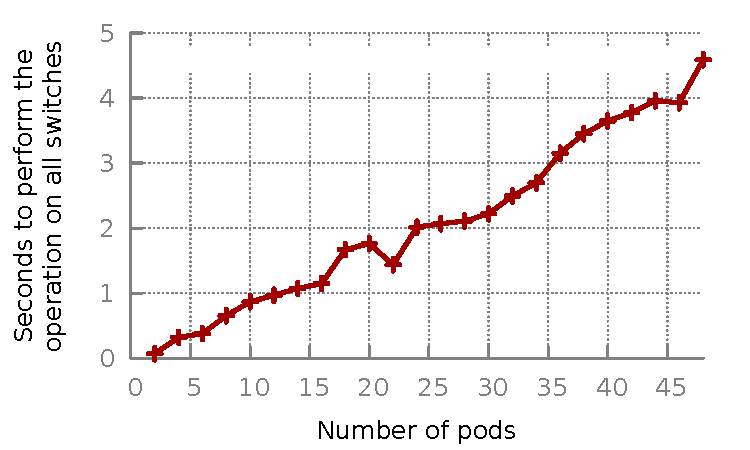
\includegraphics[width=3.25in]{../graphs/scalability_graph/scale.pdf}
    \caption[]{\label{fig:scalability} Time to send and process messages
    between controller and simulated switches. Each datapoint consists of
    $x^3/4$ hosts and $5x^2/4$ switches (\eg{} 48 pods means 27,468 hosts
    attached to 2,880 switches)}
\end{figure}

We also tested the extreme limits of the simulator's scalability, pushing up
the number of switches until something broke. We encountered what appears to be
a limitation of the Linux TCP/IP stack: TCP connection attempts began failing
beyond 26,680 sockets. Note that 26,680 switches is an order-of-magnitude larger than
the today's biggest networks.

\subsection{Replay fidelity}

On the one hand, since the SDN platform is in software, we can, in theory,
reproduce all software-induced policy violations (though not problems
resulting from flaky hardware implementing code incorrectly). However, this
requires setting up the simulator to emulate the appropriate conditions that
led to the policy violation, and that can be quite difficult. We hope to make
progress in this area along two dimensions.  First, we hope to help the
community build up a set of regression tests, so that a wide variety of
bug-triggering scenarios are available in a public repository. This would go a
long way towards providing adequate test coverage.

Second, we hope to gather error logs from real production deployments which
will help us populate this repository; this may require providing novel kinds
of anonymization, so that large datacenter operators would be willing to share
their problems (since they want their SDN code to work) without revealing the
details of their network.  This may require a infrastructural counterpart to
minimally-causal events; the smallest number of infrastructure components that
can reproduce the same bug.

Also, note that our correspondence checking algorithm can not verify
time-dependent policies such as ``No link should be congested more than 1\% of
the
time'', or ``No server should receive more than 500MB/s of external traffic''.
In future work we will extend our correspondence checking algorithm to
account for this class of policies.

\colin{reviewer B: in fact, in addition to temporal properties, the
correspondence checking algorithm cannot verify any properties involving
individual links since it only accounts for externally observable behavior!}

}
